\documentclass{beamer}
\usepackage{mathtools}
\DeclarePairedDelimiter{\ceil}{\lceil}{\rceil}
\usepackage{algorithm}
\usepackage{algpseudocode}
\usepackage[english]{babel}
\usepackage[utf8]{inputenc}
\usetheme{Madrid}
\usecolortheme{dolphin}

\logo{\includegraphics[width=0.1\textwidth]{sdu_segl}}

\title{Interaktion og interaktionsdesign}
\author{Steven Gøhler}
\begin{document}
\begin{frame}
\titlepage
Redegør for kognitive aspekter i relation til interaktionsdesign
\end{frame}

\begin{frame}
  \frametitle{Overview}
  \tableofcontents
\end{frame}

\section{Hvad er kognition?}
\begin{frame}
\frametitle{Hvad er kognition?}
  \begin{columns}[T]
    \begin{column}{.5\textwidth}
	  \begin{itemize}
		\item Opmærksomhed
		\item Opfattelse
	    \item Hukommelse
	    \item Indlæring
	    \item Sanserne
	  \end{itemize}
    \end{column}
    \begin{column}{.5\textwidth}
      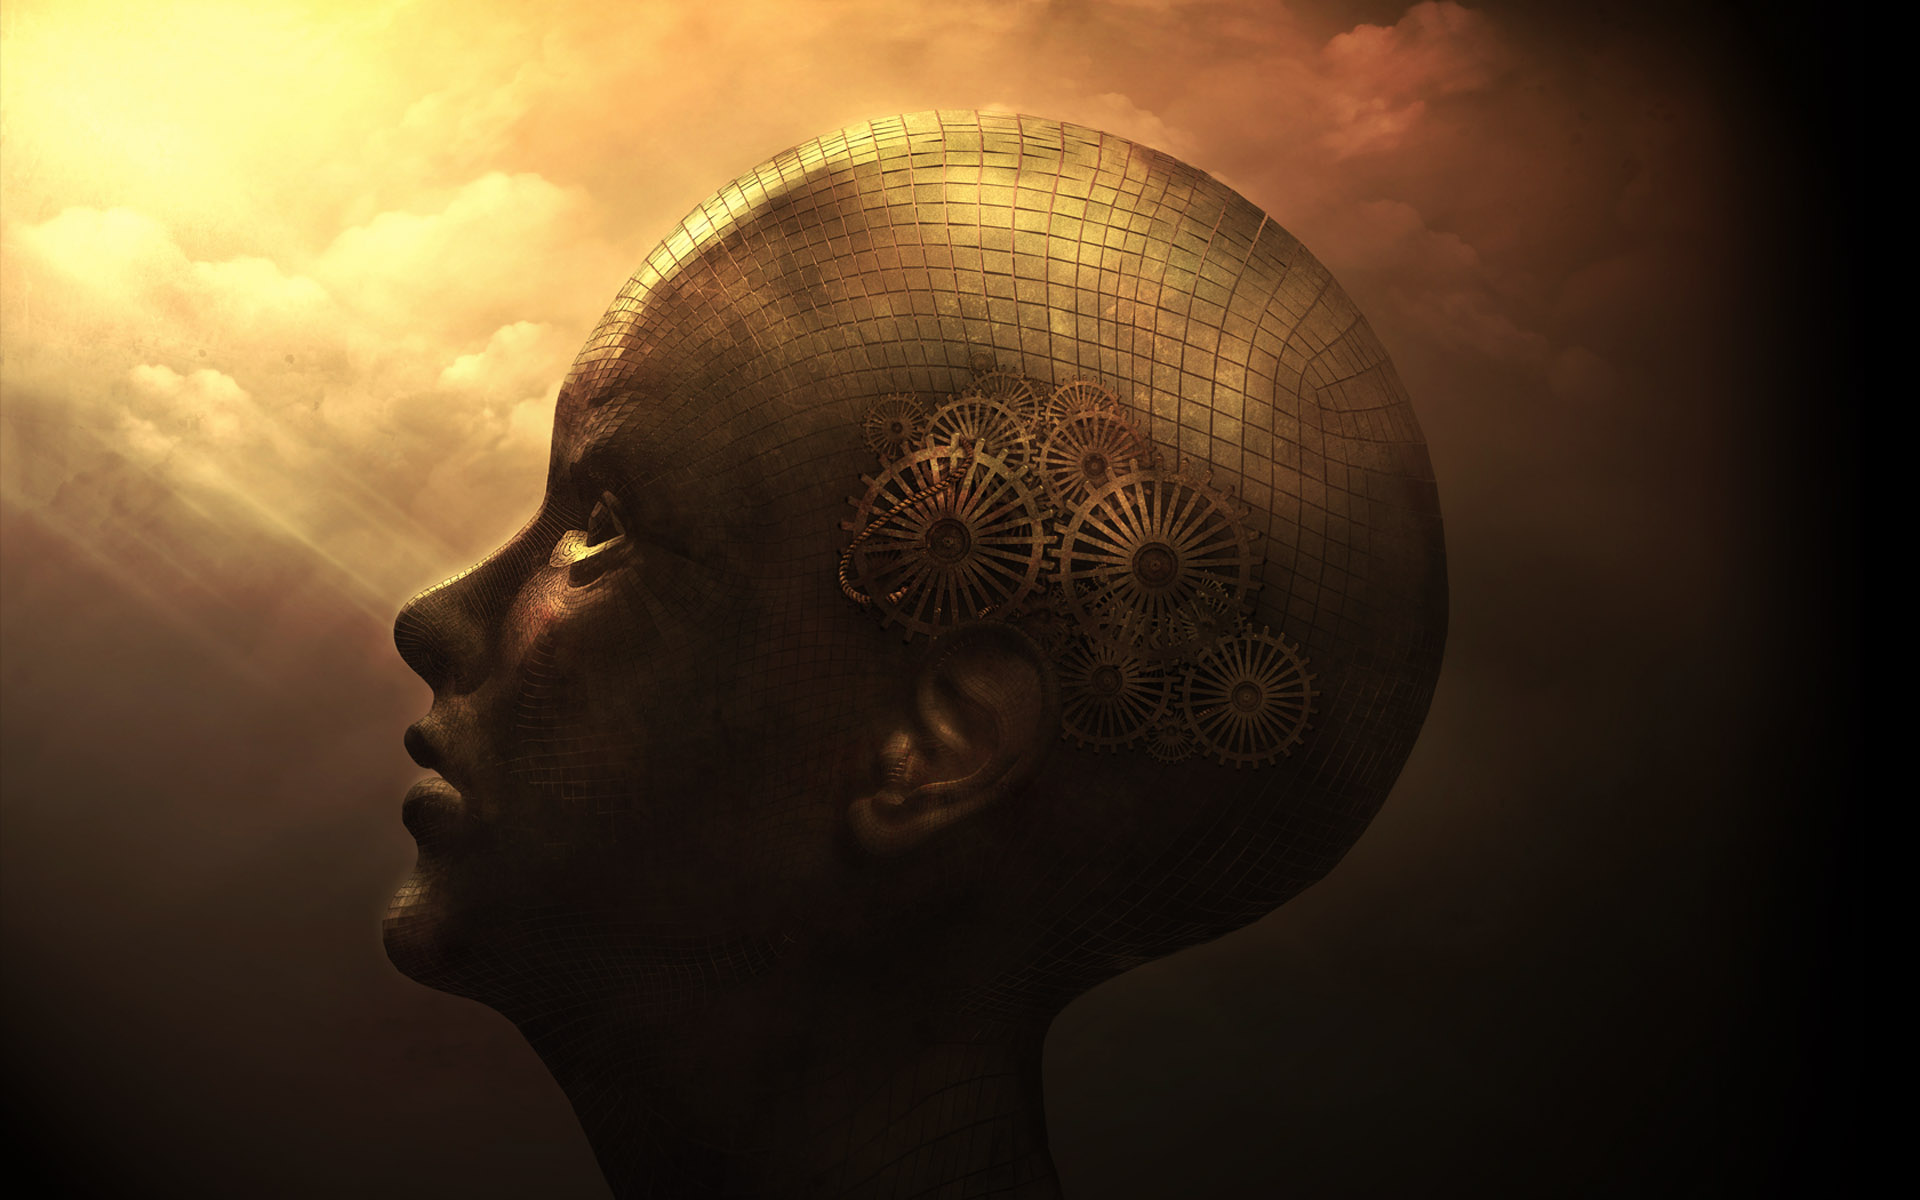
\includegraphics[width=\textwidth]{kognition.jpg}
    \end{column}
  \end{columns}
\end{frame}


\section{Opmærksomhed}
\begin{frame}
\frametitle{Opmærksomhed}
  \begin{columns}[T]
    \begin{column}{.5\textwidth}
	  \begin{itemize}
		\item Hold det simpelt
		\item Iøjnefaldende rIelevante oplysninger
	    \item Bestemte
	    \begin{itemize}
	      \item Find Holger
	      \item Find "Find Holger"
	    \end{itemize}
	    \item Overordnede
	    \begin{itemize}
	      \item Facebook
	      \item Supermarked
	    \end{itemize}
	  \end{itemize}
    \end{column}
    \begin{column}{.5\textwidth}
      
\includegraphics[width=\textwidth]{me.jpg}
    \end{column}
  \end{columns}
\end{frame}

\section{Opfattelse}
\begin{frame}
  \frametitle{Opfattelse}
  \begin{columns}[T]
    \begin{column}{0.5\textwidth}
      \begin{itemize}
	    \item Information skal opfattes på den tiltænkte måde
	    \item Grupper sammenhængende ting
	    \item Lettere at bemærke og lokalisere
	    \item Rigtige farver
      \end{itemize}  
    \end{column}
    \begin{column}{.5\textwidth}
      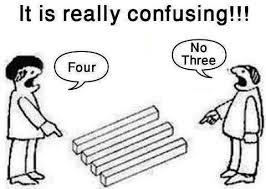
\includegraphics[width=\textwidth]{opfattelse.jpg}
    \end{column}
  \end{columns}
\end{frame}


\section{Hukommelse}
\begin{frame}
\frametitle{Hukommelse}
  \begin{columns}[T]
    \begin{column}{.5\textwidth}
	  \begin{itemize}
		\item Ram visuelle ting brugeren allerede kender	
		\item Skeuomorphism
		\item Baseret på genkendelse
	  \end{itemize}
    \end{column}
    \begin{column}{.4\textwidth}
      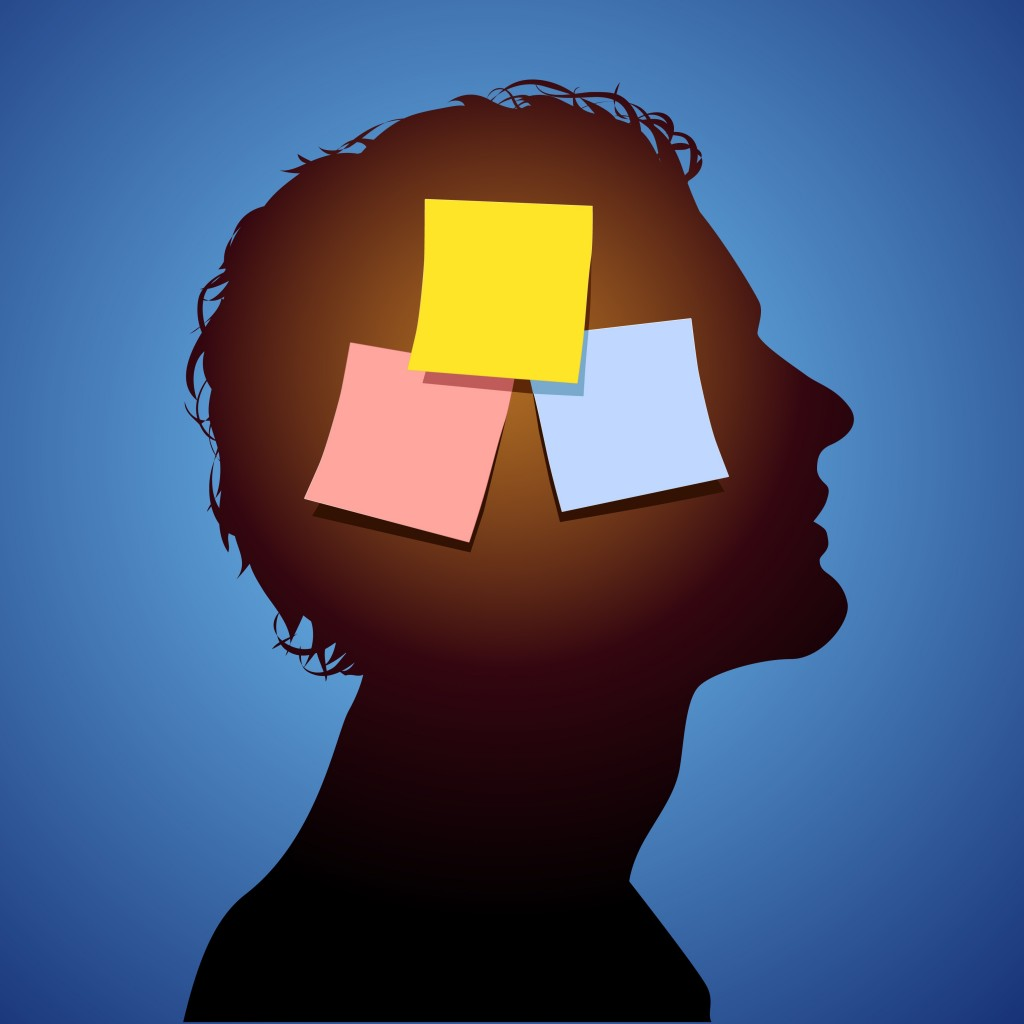
\includegraphics[width=\textwidth]{memory.jpg}
    \end{column}
  \end{columns}
\end{frame}


\section{Indlæring}
\begin{frame}
\frametitle{Indlæring}
  \begin{columns}[T]
    \begin{column}{.5\textwidth}
	  \begin{itemize}
		\item Mange indtryk
		\item Lad brugerne udforske
		\item Learning by doing
		\item Begynderguides
	  \end{itemize}
    \end{column}
    \begin{column}{.4\textwidth}
      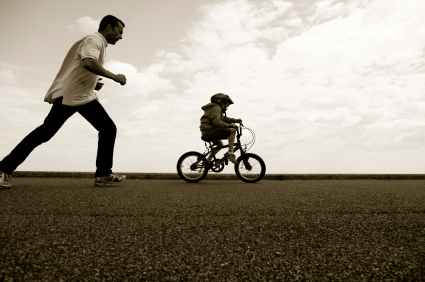
\includegraphics[width=\textwidth]{learning.jpg}
    \end{column}
  \end{columns}
\end{frame}


\end{document}